%------------------------------------------------------------------------------
%  DOCUMENT CONFIGURATION
%------------------------------------------------------------------------------

\documentclass[twoside, a4paper, titlepage]{article}

%------------------------------------------------------------------------------
%  PACKAGES
%------------------------------------------------------------------------------

\usepackage[utf8]{inputenc}
\usepackage[english]{babel}
\usepackage{csquotes} % Recommended

\usepackage{natbib}
\bibliographystyle{agsm}

\usepackage{fancyhdr} % Required for custom headers
\usepackage{lastpage} % Required to determine the last page for the footer
\usepackage{extramarks} % Required for headers and footers
\usepackage{graphicx} % Required to insert images
\usepackage{rotating} % Required for sideways figure
\usepackage{parskip} % Required for paragraph styling
\usepackage{float} % For having figures inline
\usepackage{amsmath}
\usepackage{amssymb}
\usepackage{hyperref} % For links
\usepackage{blindtext}
\usepackage{outlines}
\usepackage{tabularx}

\usepackage{minted}

\definecolor{bg}{rgb}{0.95, 0.95, 0.95}
\usemintedstyle{borland}
\usepackage{tcolorbox}
\usepackage{etoolbox}
\BeforeBeginEnvironment{minted}{\begin{tcolorbox}}%
\AfterEndEnvironment{minted}{\end{tcolorbox}}%

\usepackage{titlesec} % Used for paragraph subsubsubsection

\usepackage{tikz}
\usetikzlibrary{shapes.misc, positioning}
\restylefloat{figure}

%------------------------------------------------------------------------------

% Margins
\topmargin=-0.45in
\evensidemargin=0in
\oddsidemargin=0in
\textwidth=6.5in
\textheight=9.0in
\headsep=0.25in

% Numbering
\setcounter{secnumdepth}{4}
\titleformat{\paragraph}
{\normalfont\normalsize\bfseries}{\theparagraph}{1em}{}
\titlespacing*{\paragraph}
{0pt}{3.25ex plus 1ex minus .2ex}{1.5ex plus .2ex}

% Sans Serif Font
\renewcommand\rmdefault{cmss}

% Line spacing
\linespread{1.1}

% Images
\setlength\fboxsep{0pt}
\setlength\fboxrule{0.5pt}

\setlength\parskip{1.2em} % Space between paragraphs
\setlength\parindent{0pt} % Removes all indentation from paragraphs

% Tikz
\def\checkmark{ \tikz\fill[scale=0.4](0,.35) -- (.25,0) -- (1,.7) -- (.25,.15) -- cycle; }

%------------------------------------------------------------------------------
% TITLE PAGE
%------------------------------------------------------------------------------

\begin{document}

% Definition of blocks:
\tikzset{%
  block/.style    = {draw, thick, rectangle, minimum height = 3em,
    minimum width = 3em},
  sum/.style      = {draw, circle, node distance = 2cm}, % Adder
  input/.style    = {coordinate}, % Input
  output/.style   = {coordinate} % Output
}

\pagestyle{empty}

\newcommand{\reporttitle}{Decentralised, private, access-controlled data sharing}
\newcommand{\reportauthor}{Frederick Lindsey}
\newcommand{\reportsupervisor}{Dr. William Knottenbelt}
\newcommand{\reporttype}{BEng. Individual Project Report}

\begin{titlepage}

\newcommand{\HRule}{\rule{\linewidth}{0.5mm}}

\centering % Center remainder of the page
\vspace{1cm}


%-------------------------
%	HEADING SECTIONS
%-------------------------

\textsc{\LARGE \reporttype}\\[1.5cm]
\textsc{\Large Imperial College London}\\[0.5cm]
\textsc{\large Department of Computing}\\[0.5cm]

%--------------------------
%	TITLE SECTION
%--------------------------

\includegraphics[width = 4cm]{images/imperial_college_london_coat_of_arms}\\[0.5cm]

\HRule \\[0.4cm]
{ \huge \bfseries \reporttitle}\\
\HRule \\[1.5cm]

%--------------------------
%	AUTHOR SECTION
%--------------------------

\large
\begin{minipage}{0.5\textwidth}

\textit{Author:}\\
\reportauthor

\end{minipage}%
\begin{minipage}{0.5\textwidth}

\textit{Supervisor:}\\
\reportsupervisor

\end{minipage}

\vspace{7cm}
\makeatletter
\@date

\makeatother
\end{titlepage}


%------------------------------------------------------------------------------
% CONTENT
%------------------------------------------------------------------------------

% MOTIVATION
% CONTRIBUTIONS
% RESULTS

% APPLICABILITY
\abstract

\thispagestyle{plain}
\pagenumbering{roman}
\setcounter{page}{1}

Over the last several hundred years, the way we access and manage the world's data has radically changed. Recounting medieval times when there was little to no public record of a person's assets or information, this presents a stark comparison to today's society, where our data and identities are traded on a global market, often without our knowledge. This thesis, and it's accompanying proof of concept, seeks to describe a method of reinstating the ownership of data that was once commonplace in previous centuries, without compromising on the free flowing and global nature of communication today.

% TODO: Add information from report findings
TODO: Add information from report findings and more focused text

% Discuss motivation briefly

% Objective of determining whether a decentralised system can be successful

% Whilst possible, not ready in the slightest


% Acknowledge those who've technically or otherwise helped with completing the project
\renewcommand{\abstractname}{Acknowledgements}
\abstract

\thispagestyle{plain}
\pagenumbering{roman}
\setcounter{page}{2}

\begin{center}
  I'd like to thank Professor William Knottenbelt and Dr. Robert Learney for their support and guidance through this project. Their support was instrumental in this project and greatly appreciated.

  I'd also like to thank Professor Chris Hankin and Dr. Melek Somai for their involvement.
\end{center}


% Set up the header and footer
\pagestyle{fancy}
\pagenumbering{arabic}
% \lhead{\docAuthorName} % Top left header
\rhead{\firstxmark} % Top right header
\lfoot{\lastxmark} % Bottom left footer
\cfoot{} % Bottom center footer
\rfoot{Page\ \thepage\ of\ \pageref{LastPage}} % Bottom right footer
\renewcommand\headrulewidth{0.4pt} % Size of the header rule
\renewcommand\footrulewidth{0.4pt} % Size of the footer rule

%------------------------------------------------------------------------------
% TABLE OF CONTENTS
%------------------------------------------------------------------------------

\setcounter{tocdepth}{4}

\tableofcontents

%------------------------------------------------------------------------------
% INTRODUCTION AND PREFACE
%------------------------------------------------------------------------------

% MOTIVATION
% OBJECTIVES
% CONTRIBUTIONS
\section{Introduction}

% - Privatisation of data
%   - Google, Facebook, NHS, Banks, retail stores (loyalty programs)
%   - Data Protection Act (limitations and corporate-focus)
% - User choice (who do I want to have my data and how)
% - Online identities
%   - Global identity tracking
%   - Conglomerate identity providers
\subsection{Motivation}

Over the last 350 years, the general public has, often unwittingly, handed their right to privacy over to corporations, conglomerates, and governments. This has occurred through the exchange of personal data for the convenience of the modern world. Some might argue, however, that these transactions have not occurred in good faith and been equally beneficial to both parties.
\newline
The origin of such transactions in the UK might be attributed to the introduction of paper money in 1694 by the Bank of England~\cite{bankofengland:2016:online}. The introduction of paper currency gave an opportunity to the Bank of England to start collecting data on the exchange of money nationally. At the time it is unlikely that any person exchanging gold for paper currency was aware of the impending social shift, likely more concerned with the convenience afforded to them. Before this time, a person might have kept their savings 'under the mattress' and almost certainly would not have shared information relating to their wealth with another party. Whilst bank notes were introduced as a means to raise funds for war, the seed for a data revolution was inadvertently sewn. Whilst no unique identities were shared at this point, they would be in years to come.

Fast forward several hundred years and we find ourselves in a society where it is commonplace to rely on few key corporations and organisations to control information nationally and internationally. As (probably) the world's most popular social network~\cite{worldmapsocialnetworks:2017:online} it is clear from Facebook's terms and conditions~\cite{facebookterms:2015:online} that our use of the social network is subject to a few key conditions which restrict and change the status quo of our privacy as users. Foremost, it is apparent that whilst content posted on Facebook remains the property of the owner, Facebook has the right to use it how it wishes (as per the IP license) and hence is the controller of that data. One might choose to post it on Facebook, but one cannot stop Facebook using their content without removing it from all of Facebook's services and ensuring everyone with whom one has shared it with has also removed it from Facebook. Furthermore this allows Facebook to use any content posted for machine learning, training systems and providing commercial services using the intelligence gained from the distribution of content on the Facebook network. As someone who cares for their privacy, it is my opinion that this is not an acceptable status quo.

Notably, Facebook is not the only social network with this perspective on user privacy. Twitter also shares a very similar stance~\cite{twittertos:2017:online} and it is generally observed with most similar companies.

\begin{displayquote}{
  "\textbf{When it comes to control over our own data, health data must be where we draw the line.}"~\cite{wilbankstopol:2016:article}
}\end{displayquote}

% TODO: Swiss health identity card data

% - Privatisation of data
%   - Google, Facebook, NHS, Banks, retail stores (loyalty programs)
%   - Data Protection Act (limitations and corporate-focus)
% - User choice (who do I want to have my data and how)
% - Online identities
%   - Global identity tracking
%   - Conglomerate identity providers


At the core of the motivation for this project lay several issues corresponding to the way in which society has been manipulated over time. It is my belief that we find ourselves in the current position without any ownership of our data because we've been keen (even greedy) as a society to reap the benefits of our data without considering the longer term security effects. We have neglected our responsibility to care for our data.

Below, I have highlighted the key domains in which we lack control that we should have over our personal data. Whilst written as a piece of fiction, we should be aware and concerned that ignoring the social issues with data transfer allows a world to form much similar to that of George Orwell's 1984~\cite{orwell:1984:book} - we consider the likes of corporations synonymous with that of the 'Big Brother' character.

\subsubsection{Commoditisation of personal (and private) data}

There is no doubt that search tools such as those offered by Google and Microsoft, retail stores such as those offered by Amazon, and social networks such as Facebook and Twitter, dramatically enhance our lives and give us capabilities we would never have otherwise. Often as consumers we are eager to accept these benefits without considering the means by which they are offered to us.

% TODO: Freedom to use personal data
% \subsubsection{Freedom to use personal data}


\subsection{Objectives}

This project aims to re-imagine how we share data by prioritising the privacy, control, and availability of personal data. It is my belief that through decentralisation it is possible to have a system which no one entity controls or owns, but which every willing and able entity can participate in, privately. In the context of this project, privacy concerns the underlying data, not the transparency of data transactions occurring.

The primary objective of this project is to \textbf{discover whether a fully decentralised, private data sharing platform can exist}. The meaning of private in this context refers to hiding the content of the underlying data. The following secondary objectives follow from the primary objective:

\begin{itemize}
  \item \textbf{End-to-end Encryption} \\
  Must only share data which is encrypted and decrypted client-side. No unencrypted data flow of content is allowed.
  \item \textbf{Decentralisation} \\
  Wherever possible a decentralised service should be favoured over a centralised one.
  \item \textbf{Real-world Use} \\
  Establish whether a system would be practical for use by real people under real circumstances with real data. A practical application is central to the project's success.
  \item \textbf{Permissions} \\
  A user should be able to administer permissions for data they own
  \item \textbf{Group access} \\
  A successful implementation will allow group access under the same permissions as are available to an individual
  \item \textbf{Accessibility} \\
  The project should use technologies that can be integrated and used by current software where applicable.
\end{itemize}


\subsection{Contributions}



%------------------------------------------------------------------------------
% BACKGROUND
%------------------------------------------------------------------------------

\section{Background}

\subsection{Distributed Ledger Technology}

\subsubsection{Introduction to Distributed Ledger Technology}

Distributed ledger technology (DLT) is a recent invention which endeavours to make data publicly accessible through a decentralised system, providing no single point of failure. A DLT provides transparency where traditional centralised systems fall short and allows any willing and able party to be a part of the decentralised network. Furthermore, a DLT provides no easy way for any network moderator or specific party to control or override the network without the consensus of a significant number of the network's members. Combined, this technology introduces an entirely new way of dealing with transactional data and, as implemented below, any sort of data having a lifecycle.

\subsubsection{Blockchain}

The Blockchain~\footnote{\href{https://www.blockchain.com/}{Blockchain (https://www.blockchain.com)}} is the underlying technology that is used by cryptocurrencies such as Bitcoin~\footnote{\href{https://bitcoin.org/en/}{Bitcoin (https://bitcoin.org)}}. Since Blockchain was the first widely-available distributed ledger technology, most distributed ledger technologies since have chosen to adopt the blockchain name to refer to this architecture.

A traditional database is implemented such that it only maintains one current state for a given dataset~\footnote{Some databases have features allowing the user to view state (not transactions) over time (e.g. \href{https://www.postgresql.org/docs/6.3/static/c0503.htm}{PostgreSQL's Time Travel}) but these are not common and often deprecated} rather than transactions. In contrast, a blockchain, as the name would suggest, maintains a 'chain' of blocks of transactions that are agreed by the network forming a history of the chain's life. These blocks are formed of groups of transactions and are totally ordered across nodes in the network. It follows therefore that every node needs to have the entire history of the network, and that the provenance and origin of any given commodity, the unit of measure of a transaction, is maintained.

Whilst the above summarises the differences in the way a blockchain holds data compared to a traditional database, the differences in transaction ordering are far more fundamental and interesting. Consensus is used across a blockchain network to establish the most popular chain of transactions. It is possible for many chain possibilities to exist at any given time, but the longest chain is always assumed to be the main chain. Once a client has accepted a transaction (as part of a block), and it therefore forms part of their chain, it is not possible to choose another chain where this transaction has not been accepted (as part of the same block).

\subsubsection{Blockchain Consensus}

A few of the most popular methods of achieving consensus in a blockchain, and therefore total ordering, are listed below.

\begin{itemize}
  \item
    \textbf{Proof Of Work (PoW)}
    \textit{The majority of compute power in the network is held by honest members.~\footnote{Used by Bitcoin and Ethereum (pre-Serenity). \href{https://en.bitcoin.it/wiki/Proof_of_work}{Bitcoin Wiki}}}
  \item
    \textbf{Proof Of Stake (PoS)}
    \textit{The majority of stake (currency) in the network is held by honest members.~\footnote{Planned to be used by Ethereum (Serenity release and beyond). \href{https://www.cryptocompare.com/coins/guides/the-ethereum-releases-of-frontier-homestead-metropolis-and-serenity/}{Crypto Compare}}}
  % \item
  %   \paragraph{Byzantine Agreement (BA)}
  % \item
  %   \paragraph{Tendermint (TM)}
  % \item
  %   \paragraph{Stellar Consensus Protocol (SCP)}
\end{itemize}

\paragraph{Proof of Work}

Originally proposed as a method for countering denial of service attacks, Hashcash, authored by \cite{hashcash:1997:misc} and re-evaluated in \cite{hashcash:2002:online}, is the original proof of work scheme. The idea is that using cost-functions~\footnote{A cost-function should be parametrically expensive to compute, but efficiently verifiable. \cite{hashcash:2002:online}}, the hash of some $x$ is computed such that the left-most $n$ bits are equal to $0$. Since the hash of any two similar values is very different, as shown in program code \ref{code:example_keccak_unpredictability}, a cost-function designed in this way is difficult to compute.

\begin{listing}[H]
  \centering
  \begin{minted}{bash}
> hash('keccak256').update('Hello World!0').digest().toString('hex')
'2c6e6992915d52790a3625b459a0e7a1540a7770a6582f926d0119266b6f9f51'
> hash('keccak256').update('Hello World!1').digest().toString('hex')
'4d880de6488218d7153abeacff100608191ea63cccdd9894a602e8b3c959a276'
> hash('keccak256').update('Hello World!3').digest().toString('hex')
'f016006873889f59798ff191de74c0953892b38f77dbefc67b45af5ac705fcff'
  \end{minted}
  \caption{
    Variance between hashes of similar values
  }{
    Three similar values, shown to have very different hashes using the Keccak 256-bit hash function.
  }
  \label{code:example_keccak_unpredictability}
\end{listing}


As stated in the original Bitcoin paper (\cite{bitcoin:2008:misc}), the cryptocurrency uses Hashcash to provide block validation and to chain blocks of transactions together. As per Hashcash, the hash of the next (proposed) block must have the top $n$ bits set to zero. This value is how the network self-manages, adjusting $n$ according to a moving average of the number of blocks per hour. The hash of any particular block is computed by hashing the previous block's hash, the content of the block, and some nonce (a random value). As the nonce is incremented the hash of the block varies hugely and with sufficient iterations, the block will match the requirements of the next block.

Given the nonce we have a function difficult to compute but easy to verify, providing integrity to the underlying transactions, and ensuring that should any block be changed that's been verified, all child blocks (recursively) must be recomputed. If we assume that $51+\%$ of the compute power in the network is on honest nodes, then the longest chain will also be honest. Any malicious party would need to outpace the honest nodes in the network in order to take control and re-write the chain. The so-called $51\%$ attack is the most significant security threat to the proof-of-work model.

The proof-of-work model summarised above is used in the Bitcoin and Ethereum cryptocurrency systems for their main networks as of 15th June 2017.

\paragraph{Proof of Stake}

Intended as an alternative consensus mechanism to Proof of Work (PoW), Proof of Stake (PoS) uses a party's stake in the network to determine it's voting rights to the new block. This is in direct constrast to PoW which uses a party's compute power.

Neither Ethereum nor Bitcoin currently use proof of stake, although Ethereum is intending to use it in future releases. It remains a controversial consensus method, and as such is only summarised here.

As described by Ethereum~\footnote{\href{https://github.com/ethereum/wiki/wiki}{\textit{Ethereum Wiki}}}, there are two major consensus algorithms within the PoS category, \textbf{chain-based} and \textbf{Byzantine Fault Tolerance (BFT-style)}.

Within both of the major algorithms is the concept of a validator. A validator is someone who locks their ether as a deposit for a period of time. During this time, they are a current validator. In order to propose a block a party must be a current validator.

A chain-based algorithm uses a pseudo-random selection picking a current validator who is able to propose a block for a short time period. After this time period the validator changes. As in PoW the block proposed must point to some previously mined block, assuring a continuous chain is formed.

The BFT-style algorithm extends the idea behind the chain-based algorithm but over multiple rounds. In each round random validators are chosen to propose blocks. Over the rounds a consensus on a canonical block is reached, extending the chain.

% \paragraph{Byzantine}

% \paragraph{Stellar Consensus Protocol}

% \paragraph{Tendermint}

\subsubsection{Ethereum}

Ethereum extends the blockchain's uses beyond the direct exchange of currency and into the world whereby autonomous and publicly verifiable organisations and parties can live on the blockchain. By allowing the creation of so-called 'smart contracts', entities are established as part of the blockchain which can receive transactions from external parties (you and I). Through these transactions, the state of the contract is updated allowing the contract to function as a state transition system. Documentation and a Wiki page are the main sources of information on the Ethereum ecosystem~\footnote{\href{http://ethdocs.org/en/latest}{\textit{Read the Docs}, http://ethdocs.org/en/latest}}.

\paragraph{Ethereum Virtual Machine}

In the original blockchain, underpinning Bitcoin, a portion of every transaction is taken up by the script associated with performing it. In essence, this script represents the contract of the transaction. With Ethereum, the script transmitted with a transaction should be compatible with the Ethereum virtual machine (EVM). The EVM houses an environment where any conceivable computation of arbitrarily complexity can be achieved (turing-complete), with instructions authored and compiled in languages similar to JavaScript~\footnote{\href{https://solidity.readthedocs.io/en/develop/}{\textit{Solidity (Read the Docs)}, https://solidity.readthedocs.io/en/develop/}} and Python~\footnote{\href{https://github.com/ethereum/wiki/wiki/Serpent}{\textit{Serpent Wiki}, https://github.com/ethereum/wiki/wiki/Serpent}}. Through these languages contract code is compiled and 'activated' on an Ethereum network where it will be interacted with by externally-owned accounts (EOA). These interactions allow the realisation of the utility provided by the Ethereum network; the cryptographically secure underpinnings and distributed compute.

\paragraph{Decentralised Applications (ÐApps)}

With the EVM summarised above, we move to understanding the architecture of applications hosted by the Ethereum network and run on the EVM. A decentralised application (ÐApp) is an application whose's logic is hosted on the Ethereum network (through the medium of smart contracts) and interacting with the logic is done through a decentralised interface.

\subsubsection{Merkle Trees}

The importance of Merkle trees in the architecture and implementation of decentralised systems cannot be underestimated. When discussing the hashing of blocks above, the hash at the core of the block is that representing the integrity value of the transactions the block contains. As will be evidenced in the discussion of decentralised storage platforms, Merkle trees are at the very core of hashing the transactions in a block.

\cite{merkle:1988:inbook} authored a scheme to build trees where the content of a node could be validated as a function of the hash of other nodes. First one chooses a suitable hash function, and applies this to all leaf nodes in a possible tree. Then, one must apply the same hash function applied to the leaf nodes to the parent nodes such that every parent's hash is the hash of the sum of it's own value and the hashes of it's direct children. This structure results in a tree as in figure \ref{fig:example_merkle_tree}.

\begin{figure}[H]
  \centering
  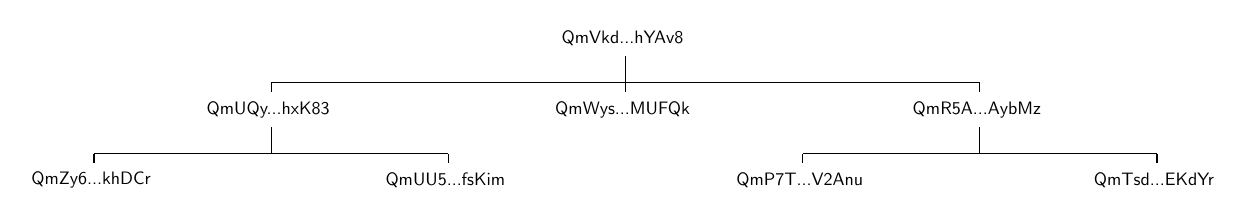
\begin{tikzpicture}[scale = 0.45, every node/.style={scale = 0.65}, every node/.append style={fill = white, rounded corners = 2pt, inner sep = 2pt, align = center}]

  \node at (0, 0) { QmVkd...hYAv8 };

  \draw (0, -0.5) -- (0, -1.5);
  \draw (-10, -1.25) -- (10, -1.25);
  \draw (-10, -1.25) -- (-10, -1.5);
  \draw (10, -1.25) -- (10, -1.5);

  \node at (-10, -2) { QmUQy...hxK83 };
  \node at (0, -2) { QmWys...MUFQk };
  \node at (10, -2) { QmR5A...AybMz };

  \draw (-10, -2.5) -- (-10, -3.25);
  \draw (-15, -3.25) -- (-5, -3.25);
  \draw (-15, -3.25) -- (-15, -3.5);
  \draw (-5, -3.25) -- (-5, -3.5);

  \draw (10, -2.5) -- (10, -3.25);
  \draw (15, -3.25) -- (5, -3.25);
  \draw (15, -3.25) -- (15, -3.5);
  \draw (5, -3.25) -- (5, -3.5);

  \node at (-15, -4) { QmZy6...khDCr };
  \node at (-5, -4) { QmUU5...fsKim };

  \node at (5, -4) { QmP7T...V2Anu };
  \node at (15, -4) { QmTsd...EKdYr };

  \end{tikzpicture}
  \caption{
    Example merkle tree
  }
  \label{fig:example_merkle_tree}
\end{figure}



\subsection{Proxy Re-Encryption}

\subsubsection{Introduction to Proxy Re-Encryption}

\begin{displayquote}{
  \textbf{"In a proxy re-encryption scheme a semi-trusted proxy converts a ciphertext for Alice into a ciphertext for Bob without seeing the underlying plaintext"}~\cite{greenateniese:2006:article}
}\end{displayquote}

Introduced as 'atomic proxy cryptography'~\cite{bbs:1998:book}, proxy re-encryption is the process of taking a message $M_a$, encrypted for a party $P_a$, and re-encrypting it such that it is readable by party $P_b$. Through the re-encryption process, the message is never decrypted by the proxy, such that the data is never revealed to any parties (including the proxy) other than the delegator and delegatees. This process relies on the functional relationship between the two ciphertexts, with the characteristics of the proxy re-encryption processed determined by the topology of this function.

\begin{figure}[H]
  \centering
  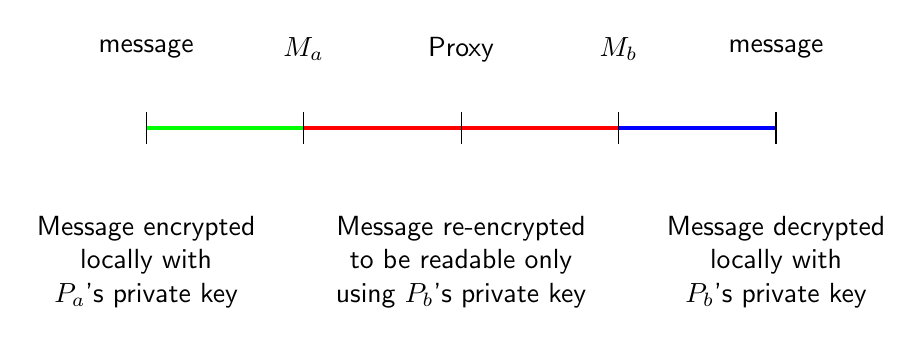
\begin{tikzpicture}

  \node at (0, 1)   {message} ;
  \node at (2, 1)   {$M_a$}   ;
  \node at (4, 1)   {Proxy}   ;
  \node at (6, 1)   {$M_b$}   ;
  \node at (8, 1)   {message} ;

  \draw [very thick, green] (0,0)   -- (2,0)   ;
  \draw [very thick, red]   (2,0)   -- (6,0)   ;
  \draw [very thick, blue]  (6,0)   -- (8,0)   ;
  \draw                     (0,-.2) -- (0, .2) ;
  \draw                     (2,-.2) -- (2, .2) ;
  \draw                     (4,-.2) -- (4, .2) ;
  \draw                     (6,-.2) -- (6, .2) ;
  \draw                     (8,-.2) -- (8, .2) ;

  \node[align=center, below] at (0, -1)%
    {Message encrypted\\locally with\\$P_a$'s private key};
  \node[align=center, below] at (4, -1)%
    {Message re-encrypted\\to be readable only\\using $P_b$'s private key};
  \node[align=center, below] at (8, -1)%
    {Message decrypted\\locally with\\$P_b$'s private key};

  \end{tikzpicture}
  \caption{
    Journey of a message using a proxy re-encryption scheme.
  }
\end{figure}


In figure \ref{fig:pre_example}, whether data is handled or manipulated by a fully trusted entity (a delegator or delegatee) or not is indicated using green/blue and red lines respectively.

The encrypted message $M_a$ is passed to the semi-trusted proxy along with the re-encryption key ( some $f(SK_a, PK_b)$\footnote{$SK_x$ represents the secret (private) key of a party $x$, $PK_x$ represents the public key of a party $x$.})

Below I discuss the contributions of various authors through the history of proxy re-encryption and the available schemes that might be suitable for a project focused on providing secure data sharing and storage.

% Delegation – allows a message recipient (keyholder) to generate a re-encryption key based on his secret key and the key of the delegated user. This re-encryption key is used by the proxy as input to the re-encryption function, which is executed by the proxy to translate ciphertexts to the delegated user's key. Asymmetric proxy re-encryption schemes come in bi-directional and uni-directional varieties.

% - In a bi-directional scheme, the re-encryption scheme is reversible—that is, the re-encryption key can be used to translate messages from Bob to Charlie, as well as from Charlie to Bob. This can have various security consequences, depending on the application. One notable characteristic of bi-directional schemes is that both the delegator and delegated party (e.g., Charlie and Bob) must combine their secret keys to produce the re-encryption key.
% - A uni-directional scheme is effectively one-way; messages can be re-encrypted from Bob to Charlie, but not the reverse. Uni-directional schemes can be constructed such that the delegated party need not reveal its secret key. For example, Bob could delegate to Charlie by combining his secret key with Charlie's public key.

% Transitivity – Transitive proxy re-encryption schemes allow for a ciphertext to be re-encrypted an unlimited number of times. For example, a ciphertext might be re-encrypted from Bob to Charlie, and then again from Charlie to David and so on. Non-transitive schemes allow for only one (or a limited number) of re-encryptions on a given ciphertext. Currently, there is no known uni-directional, transitive proxy re-encryption scheme. It is an open problem as to whether such constructions are possible.

\subsubsection{Atomic Proxy Cryptography}

Recognising that it is intuitive to expect any good cryptography scheme to disallow any untrusted party to re-encrypt a ciphertext, \cite{bbs:1998:book} suggests that perhaps it is desirable to allow re-encryption of a ciphertext, but only for specific delegatees. This is subject to doing so atomically, i.e. without revealing the underlying ciphertext, and without knowledge of the delegator or delegatee being exposed in the process. Conceptually this means that a delegator can encrypt once and have semi-trusted proxies re-encrypt for delegatees when desired.

Let's suppose we have a cryptography scheme whereby the following functions are observed:

\begin{itemize}
  \item $Gen(...)$: A generator of keys requiring arbitrary arguments
  \item $Encrypt(m, k)$: Allows the encryption of a message $m$ using the $k$ such that it is only decryptable by it's counterpart (or itself, if symmetric)
  \item $Decrypt(m, k)$: Allows the decryption of some encrypted message $m$ using the key $k$. Successful only if the message $m$ was encrypted (and intended for) the owner of the key $k$.
  \item $\Pi(m, rek_{a \rightarrow b})$: Allows the re-encryption of some encrypted message $m$ intended for the owner of key $a$ such that it is decryptable by the owner of key $b$.
  \item $ReGen(..., SK_a, PK_b)$: A generator of re-encryption keys requiring arbitrary arguments including keys required to decrypt
\end{itemize}}

As an example, imagine you wished to share an image privately between several friends. You encrypt this image and generate re-encryption keys for your friends (delegatees). Publishing the image and the keys means any third party (including the friends themselves) are able to re-encrypt the encrypted image such that a delegatee is able to decrypt it and view it.

The importance of the re-encryption function being atomic cannot be understated. The re-encryption function $\Pi$ alters the ciphertext effectively performing $\Pi(m_a, RK_{a \rightarrow b}) = Encrypt(Decrypt(m_a, SK_a), PK_b)$. However, if $\Pi$ were not atomic, the decryption of the message $m_a$ would reveal the plaintext content of the message to the proxy.

The following trust axioms apply to proxy re-encryption (assuming perfect implementation). The latter axiom only applies to symmetric key cryptography. Since the latter axiom is an undesirable property, we seek to only use asymmetric (public-key) cryptography to maintain security (of both parties).

\begin{itemize}
  \item A (unconditionally) trusts B since B can decrypt on behalf of A
  \item B trusts A since A can calculate $SK_b$ using the proxy key and $SK_a$. (\textit{Symmetric keys only})
\end{itemize}}

Given these properties, we will assume that asymmetric cryptography is a requirement of proxy re-encryption going forward.

\cite{bbs:1998:book} also discusses the notion of active versus passive proxy schemes distinguishing whether the delegatee has to cooperate or not in the creation of the proxy key. In practice, if the delegatee's public key is made available and is the only requirement from the delegatee then the delegator can delegate without the delegatee present, but otherwise, e.g. if the delegatee's secret key is required, the delegator needs the delegatee's cooperation to generate the proxy key required. Furthermore, in consideration of the delegator and delegatee's personally-identifying information, the proxy key can be distinguished as being transparent, translucent, or opaque depending on the ability of a third party to distinguish the two public keys the proxy is re-encrypting between.

\paragraph{El Gamal Cryptography}

\cite{bbs:1998:book} uses El Gamal encryption~\cite{elgamal:1985:article} as the basis for the proxy cryptography scheme suggested. A brief description of the protocol follows.

The El Gamal scheme includes the following functions:

% TODO: Clarify
\begin{itemize}
  \item $Gen(..., g, Zn)$: A generator of keys requiring arbitrary arguments including some $g$, a generator in $Zn$, itself a finite cyclic group of order $n$. Produces some secret key $\alpha$, whereby $0 \le \alpha \le n$, and a public key $g^\alpha$.
  \item $Encrypt(m, pk)$: Takes a random number, $r$. Encrypts a message $m$ using the shared secret represented by $g^a^r = k$, A's public key to some random power. Outputs the tuple $(g^r, mk mod n)$.
  \item $Decrypt(<pk, c>, sk)$: Decrypts some encrypted message $c$ using the secret key $sk$. Successful only if the message $c$ was encrypted for the owner of the key $sk$.
\end{itemize}

It is based on the Diffie-Helman protocol and relies on the discrete logarithm problem of $A = g^a$ being difficult.

\subsubsection{Proxy Cryptography Revisited~\cite{ivandodis:2003:inproceedings}}

\subsubsection{Improved Proxy Re-encryption Schemes with Applications to Secure Distributed Storage~\cite{afgh:2006:article}}

\subsubsection{Unidirectional Chosen-Ciphertext Secure Proxy Re-Encryption~\cite{lv11:2011:article}}


\subsection{Off-chain storage}

Whilst the storage of data is well researched, since the aim of this project is to evaluate the applicability of new and immature software to solve key social and technological challenges, there is an opportunity to discover up and coming technology in the storage space.

When using blockchain as the central data lake for an application, we must consider where we store the data that it references. Whilst is is possible to store data on blockchain itself, it is impractical and extremely expensive as discussed below. Storing data on the chain, assuming a transaction will be accepted on Ethereum with a gas price of 0.2 microether, at the current prices~\footnote{\$244.96 / ETH as of 4th June 2017. Breakdown of transaction costs at \href{https://www.cryptocompare.com/coins/guides/what-is-the-gas-in-ethereum/}{Crypto Currency}}, correlates to a cost of 263,023.8 USD per GB.

$$
\begin{aligned}
5 * 1024^{3} * 0.2 * 10^{-6} &=& 1,073.74 \text{ ETH (2sf)} \\
&=& 263,023.80 \text{ USD (2sf)}
\end{aligned}
$$

Bear in mind that I have ignored other transaction costs, including submitting and storing execution cycles, and indeed a limit on block size exists on Ethereum~\footnote{\href{https://ethstats.net/}{EthStats} showed a gas limit of the order of 4.7 million as of 5th June 2017.}. Henceforth it is trivial that it would be inappropriate to store any data on blockchain other than that which represents state of the application.

To solve this issue, we therefore need to assume that data needs to be stored by some other manner such that it is readily available, but only addressed (not stored) in blockchain. Below are two solutions.

\subsubsection{Centralised data storage}

There are many incumbents in the data storage market offering centralised, redundant data platforms. The most popular at the time include \href{https://aws.amazon.com/s3/}{Amazon Web Services S3}, \href{https://cloud.google.com/storage/}{Google Cloud Storage}, and \href{https://azure.microsoft.com/en-gb/services/storage/}{Microsoft Azure Storage} to name a few. Whilst the specific storage prices for each service are not relevant, each provider offers the storage at a rate of the order of less than 0.1 USD / GB / month. Even if we imagine that the storage offered by Ethereum would remain persistent and accessible for fifty years, the cost of storage on modern centralised data storage platforms is of the order of more than four thousand times cheaper. 

It is not within the scope of this report to consider the performance benefits of different cloud providers and their individual architectures. None of the big players in the centralised data storage market offer similarly performant decentralised solutions that would be useful in the context of this project.

\subsubsection{Decentralised data storage}

Decentralised storage, using peer-to-peer networks for data flow, represents an interesting and novel approach for data storage. Until recently, the only commonly used peer-to-peer data storage was that of torrents. Some software providers~\footnote{Canonical provide images of their Ubuntu operating system available through torrent files. \href{https://www.ubuntu.com/download/alternative-downloads}{Ubuntu Alternative Downloads}} have made free software available through this medium before, although historically the use of torrents for mainstream content sharing has been limited to illegal activities largely involving the use of copyrighted material.

In more recent times, more modern implementations of peer-to-peer storage have arisen. The Inter-planetary File System~\footnote{IPFS is aiming to replace HTTP as the protocol we use to access data. \href{https://ipfs.io/}{\textit{IPFS is the distributed web}}} (IPFS) and Storj~\footnote{Storj aims to provide a decentralised and encrypted platform for sharing data. } are two options that somewhat extent the concept of peer-to-peer sharing through torrenting.

\paragraph{IPFS}

IPFS takes the peer-to-peer nature of torrenting and wraps it in a application and caching layers to provide a high-performance decentralised storage solution with the following benefits.

\begin{itemize}
	\item 
    	\textbf{Content-based addressing} \\
        All content sent to the IPFS network is addressed as part of a Merkle tree (tree of hashes) such that the integrity of the content can be validated by the hash, and that the hash (address) remains constant with the content.
    \item 
    	\textbf{Local storage of data (content)} \\
        An IPFS node caches hashes which are requested such that it can provide them more quickly to nearby peers including repeated requests by the owner of the node for the same hash.
    \item 
    	\textbf{Permanent Web} \\
        Due to the decentralised nature of IPFS, and the above content-based addressing, once a blob is present on the network, it cannot be revoked without all nodes which hold a copy deleting it. For content which has not yet been requested by any other node than the one where it was created, deletion might be possible, but it should be considered that IPFS represents somewhat permanent storage.
    \item
    	\textbf{Offline Web} \\
        IPFS provides the means for offline, localised websites and storage. Rather than requiring the backbone of the internet to provide connectivity between peers, local area networks of IPFS nodes are able to communicate and share data without barriers.
\end{itemize}

\paragraph{Storj}

Pronounced 'storage', Storj leverages it's own  cryptocurrency



%------------------------------------------------------------------------------
% DESIGN
%------------------------------------------------------------------------------


% TODO: Research

%------------------------------------------------------------------------------
% IMPLEMENTATION
%------------------------------------------------------------------------------

\section{Implementation Considerations}

\subsection{Encrypting Data}

\subsubsection{Choosing A Cryptography Scheme}

Fundamental to this project is the underlying end-to-end encryption of data. Without end-to-end encryption this project represents nothing more than a public ledger of the distribution of the files belonging to an identity, readable by any party. Henceforth, choosing a suitable and secure cryptography scheme is critical.

Firstly, an asymmetric cryptography scheme with a public-private key pair is required in order to facilitate proxy re-encryption. As the most popular scheme~\footnote{As used in SSL encryption globally} RSA~\cite{rsa:1978:article} seemed a suitable candidate. Whilst the proxy re-encryption scheme authored by \cite{afgh:2006:article} meets many more desirable properties than that authored by \cite{ivandodis:2003:inproceedings}, the appeal of using a well-studied cryptography scheme to underpin the resulting application was thought to be more important. This was reinforced by the 


\subsubsection{Applying Proxy Re-encryption}



\subsection{Ethereum}

\subsubsection{Micro Architecture}

Distributed ledger technology is at the very core of any decentralised project. In this project, it provides the compute backbone, the only non-local, stateful system in the project architecture. Whilst this compute backbone has, until now, been observed as a monolithic module, we now consider it's implementation and own micro-architecture.

It is trivial that every identity, every user of the proposed system, needs to have their own state representative of files they own and associated metadata. It is also trivial that every group that exists on the network must exist as a collection of identities and this should exist as some state along with associated metadata. We therefore need two contracts, as a minimum, each representative of some state. These will be called the 'Storage' contract and the 'Group' contract.

However, these two contracts will be instantiated in arbitrary sizes. Upon launch of a system, there would be zero of either, but with user adoption will come contract instantiation. 

\paragraph{Storage Contract}

\paragraph{Group Contract}

\paragraph{Registry Contract}

% TODO: Get to the below diagram

\input{tikz/architecture/ethereum_micro_architecture}

Figure \ref{fig:ethereum_micro_architecture}



\subsection{Permission Layering}

\subsubsection{Individual Permissions}

For the purposes of this section, an individual refers to an individual identity. This may be held by an organisation or by a person, and is someone to whom the data owner directly gives permissions.

There are several considerations to make when giving another identity permissions:

\begin{itemize}
  \item 
  	\textbf{Access Control} \\
    The ability of an individual to get access to the location of a file
  \item
  	\textbf{Read} \\
    The ability of an individual to read the contents of a file, correctly.
  \item
    \textbf{Write} \\
    The ability of an individual to write the contents of a file, correctly.
\end{itemize}

\paragraph{Access Control}

A simple permissions system based on basic UNIX ACL (access control list) permissions is used, allowing a number $x$ in the range of $[0..2^n)$ where $n$ represents the number of permission types available (read, write, etc.). $x$ models the permissions for a given identity. This project only requires primitive permissions to show proof of concept, those permissions being only 'read' and 'write'. Given these two possibilities there are four possible permission settings per identity:

\begin{table}[H]
  \centering
  \begin{tabular}{ | l | c | c | }
    \hline
    Number & Read & Write \\
    \hline
    0 & & \\
    1 & \checkmark & \\
    2 & & \checkmark \\
    3 & \checkmark & \checkmark \\
    \hline
  \end{tabular}
  \caption{
  	Identity permission modeling
  }{
    The four possible permissions settings an identity could have at any given time. Each setting is mutually exclusive of any other.
  }
  \label{table:pre_properties}
\end{table}

Given the settings in table it is easy to understand whether any identity has a given permission. Let's imagine a system that has $n = 20$, and we wish to understand if a particular identity, with permissions $x$, has permission $14$ set. We apply the following function:

\input{code/StoragePermissionsCheck.tex}

The function shown in figure \ref{code:storage_permissions_check} is derived from the fact that a permission $n$ is represented by the $n-1^{\text{th}}$ bit, such that if all possible permissions were set for a given user, $x = 2^{n} - 1$. 


\subsubsection{Group Permissions}

\paragraph{Extending Individual Access Control}

Group permissions extend the above system for individual permissions and require the use of smart contracts.

Whilst our application is intended to be fully decentralised, the key stakeholders for some applications (such as health care) may require access to the network to administrate. One example of this is the involvement of the GMC in validating doctor identities. If a doctor has not been registered, or has been struck off, they should not have any access to patient data (even if they claim to be a doctor). They should only have access should the GMC validate that they are in fact a valid doctor.

The idea of a group administrator, such as the GMC, conflicts with the idea of the data owner maintaining full access control and administration. However, should the data owner decide that the group should no longer have any access or wishes to change group permissions, they are able to do so.

To facilitate this, let's take a look at the architecture of a group's interactions with a particular identity's contract.

\input{tikz/architecture/group_interactions}

An identity claiming to be a member of a group will always interact with the storage contract it is trying to retrieve from or add data to. A group itself will never be able to directly affect or transact with a storage contract such that no malicious attacker would be able to pseudo-anonymously act as the group.

When the identity tries to access a path, their identity is cross-checked with the group they claim to be a member of. Should this group validate the identity as a member, and assuming the group has the necessary permissions that are required to action the identity's transaction, the transaction will be successful.

\paragraph{Group Key Sharing}

Whilst the process of writing data is similar to an individual (other than the membership validation above), the process of reading data differs hugely for groups.

If we were to extend the process of reading as an individual to a group, the result would be a process similar to that shown in figure \ref{fig:encryption_group_read_theoretical}.

\input{tikz/encryption/group_read}

Given the non-transitive nature of the proxy re-encryption scheme we are using, the process shown in figure \ref{fig:encryption_group_read_theoretical} doesn't allow end-to-end encryption. After the first stage of re-encryption, $\text{Data}_{G}$ represents a first-level encryption under the group $G$'s public key. Since the proxy re-encryption scheme being used only allows re-encryption from a second-level encryption to a first-level encryption (to eliminate transitivity), no further action is possible. Another process is required to facilitate group read.

If only one re-encryption is possible, the identity we re-encrypted for becomes the main priority. We ask ourselves whether the original (individual) scheme could work here, and indeed it could, although it comes with flaws described below.

\begin{itemize}
  \item
  	\textbf{Non-optimal key storage} \\
    For every member of the group, a re-encryption key must be generated by the storage contract owner. The process of generating a re-encryption key for every member is $O(n)$, i.e. for a group with a membership of 50, 50 re-encryption keys need to be generated.
  \item
  	\textbf{Interaction: Member joins} \\
    When a member joins the group, the storage contract owner is required to generate a re-encryption key for the member such that the member can read data
  \item
  	\textbf{Interaction: Member leaves} \\
    When a member leaves the group, the storage contract owner must revoke the re-encryption key generated for the user. Since there may be a time difference between the group removing the member and the storage contract owner revoking the re-encryption key, this difference is exploitable by the member.
\end{itemize}

As an improvement to individual keys, let's take another look at the viability of the theoretical group read process.

Let's assume that there is a group key pair (specifically for encryption). When a member of the group requests data from a storage contract, they receive the data encrypted for the storage contract owner and a re-encryption key $re_{SCO \rightarrow G}$. They are able to use this pair to re-encrypt the data received to be $D_{G}$.

\input{tikz/encryption/group_read_practical}

The following now apply:

\begin{itemize}
  \item The data is encrypted such that the group private key is required to decrypt it
  \item The group private key is encrypted using the group public key such that it can only be decrypted by itself
  \item The administrator $A$ of the group $G$ must have a re-encryption key $re_{G \rightarrow A}$ available such that they can create further re-encryption keys and manage the group.
\end{itemize}

When a member joins the group, the administrator creates a re-encryption key for them such that they are able to re-encrypt and then decrypt the group's private key. However, when a member leaves the group, the reference to their re-encryption key is removed from the group contract. It is likely that the group administrator would want to create a new key pair when a member leaves, to ensure no valuable data can be kept (encryption or re-encryption keys). Once the previous key pair has been invalidated a re-encryption key must be generated by the storage contract owner, requiring a level of interactivity between a group and a storage contract owner.

In contrast to figure \ref{fig:encryption_group_read_theoretical}, the process of receiving data as a member of the group now follows a process similar to that shown in figure \ref{fig:encryption_group_read_practical}.

Whilst the differences in the two schemes for group key sharing above are subtle, their differences become apparent when considered at scale.

\begin{table}[H]
  \centering

  \textbf{Giving Read Permission} \\
  \begin{tabular}{ | l | c | c | c | }
    \hline
    No. Storage Contract & Group Membership & Scheme 1 & Scheme 2 \\
    \hline
    1 & 50 & 50 & 51 \\
    10 & 50 & 500 & 60 \\
    100,000 & 100,000 & $10^{10}$ & 200,000 \\
    \hline
  \end{tabular}

  \vspace{5mm}

  \textbf{Revoking Read Permission} \\
  \begin{tabular}{ | l | c | c | c | }
    \hline
    No. Storage Contract & Group Membership & Scheme 1 & Scheme 2 \\
    \hline
    1 & 50 & 50 & 1 \\
    10 & 50 & 500 & 10 \\
    100,000 & 100,000 & $10^{10}$ & 100,000 \\
    \hline
  \end{tabular}

  \vspace{5mm}

  \textbf{Member Joins} \\
  \begin{tabular}{ | l | c | c | c | }
    \hline
    No. Storage Contract & Group Membership & Scheme 1 & Scheme 2 \\
    \hline
    1 & 50 & 1 & 1 \\
    10 & 50 & 10 & 1 \\
    100,000 & 100,000 & 100,000 & 1 \\
    \hline
  \end{tabular}

  \vspace{5mm}

  \textbf{Member Leaves} \\
  \begin{tabular}{ | l | c | c | c | }
    \hline
    No. Storage Contract & Group Membership & Scheme 1 & Scheme 2 \\
    \hline
    1 & 50 & 1 & 51 \\
    10 & 50 & 10 & 60 \\
    100,000 & 100,000 & 100,000 & 200,000 \\
    \hline
  \end{tabular}

  \caption{
    Comparison of group key sharing scheme complexity
  }{
    A comparison between schemes whereby the storage contract owner and the group administrator are required to distribute re-encryption keys. Comparison over the number of storage contracts an arbitrary group can read from, with membership as shown.
  }
  \label{table:group_key_sharing_scheme_comparison}
\end{table}

Table \ref{table:group_key_sharing_scheme_comparison} shows the huge difference in complexity of the two schemes. We take $n$ as the number of storage contracts for which the group has read permissions, and $m$ as the group membership. 

The former scheme (scheme 1 above), modeled on individual permissions, has a complexity of $O(n \times m)$ for giving / revoking read permission - each storage contract owner must create / revoke a re-encryption key for every member of the group. When a member joins / leaves a group, each storage contract owner must create / revoke a re-encryption key, $O(n)$.

The latter scheme (scheme 2 above), segregating group and member key management, has a complexity of $O(n + m)$ for giving read permission or a member leaving - each storage contract owner must create a (new) re-encryption key for the group, with the group administrator responsible for re-encryption keys for the members. When a storage contract owner revokes the group's read permission they only need to revoke the group's re-encryption key $O(1)$ per storage contract owner. When a member leaves, regardless of the number of storage contracts it affects, revoking their access is $O(1)$.

In context of the health care use case of this project, the difference between the above complexities decides the success of a project. Since the latter scheme has a lower upper bound for complexity of $O(n + m)$ over its set of operations, in a health care scenario, it would be advisable that groups are sufficiently large to cover the most likely of circumstances, but not too large that a change in membership incurs a heavy computational cost.



\subsection{Data Layering}

We have a system which is able to support end-to-end encryption of data with permissions and access control. As an extension of this, we briefly consider how this data might be layered such that different parties see different views of data.

As an example, take the following JSON object in program code \ref{code:patient_record_json}. Let's assume this represents a record of a patient visiting a general practitioner.

\begin{listing}[H]
  \centering
  \begin{minted}{json}
{
  "doctor": {
    "id": 01234567,
    "name": "Dr. So So"
  },
  "metadata": {
    "created": "2017-01-01T10:05:00+00:00",
    "modified": "2017-01-01T10:11:12+00:00"
  },
  "notes": "..."
}
  \end{minted}
  \caption{
  	An example patient record
  }
  \label{code:patient_record_json}
\end{listing}


Now let's split the JSON object into three further JSON objects corresponding to the "doctor", "metadata", and "notes" properties. We could also do the same to the "doctor" and "metadata" objects. This would result in five separate JSON objects which, when combined, form the original JSON object. This is a recursively applied process.

\subsubsection{Storing data chunks}

Since the structure of a JSON object is representative of a tree, when evaluated as above, we can use this property to visualise the data as a file system:

\begin{listing}[H]
  \centering
  \begin{minted}{bash}
file.json
├── doctor.json.part
│ ├── id.json.part
│ └── name.json.part
├── metadata.json.part
│ ├── created.json.part
│ └── modified.json.part
└── notes.json.part

2 directories, 5 files
  \end{minted}
  \caption{
    JSON represented as a file structure
  }
  \label{code:json_file_structure}
\end{listing}

\subsubsection{Permissions for data chunks}



%------------------------------------------------------------------------------
% OPTIMISATION
%------------------------------------------------------------------------------

\include{sections/05_optimisation}

%------------------------------------------------------------------------------
% CONCLUSION
%------------------------------------------------------------------------------

\section{Conclusion and Future Work}

This thesis set out to investigate the viability of a decentralised, secure, data-sharing platform. In doing so, multiple solutions have been considered and has resulted in a proof of concept being developed. One of the core objectives was to challenge the compromises users make by being actors in centralised data-sharing services, prolific globally. Through this lay the challenge of adapting new and up and coming technologies and progressing our understanding of their abilities.

This thesis shows that a secure, decentralised platform for data sharing can exist and affords its users considerable benefits over traditional centralised systems. This requires a single pair of keypairs (identity and encryption) and allows a completely secure system, whilst not imposing any more responsibility on the user than normal. Through the way the Web3 technologies interface with current browsers and computing systems, accessibility is maximised given the technology available.

It would be incorrect to say that the current implementation and work done is final. However, within the time contraints of the project, much work has been done to prove that a decentralised system can work and to discover some of the problems of designing and implementing such a system. Of most importance, the layered access system through group and individual key exchange. Secondly, this project represents the first public practical use of proxy re-encryption that I am aware of - other uses including commercial database products. Thirdly, the combination of decentralised compute and decentralised storage providing a system that is usable globally under different network conditions.

Whilst there are areas of concern which can be solved in future works, this investigation has been successful with a strongly positive outcome.

\subsection{Future Work}

Having considered the progress of this project in meeting its objectives, I'd like to suggest some key areas where further work would achieve significant improvement.

\subsubsection{Further investigation of proxy re-encryption}

Proxy re-encryption has been used in this project to answer the question of whether truly decentralised privacy and data sharing can exist. In this way proxy re-encryption acts as a facilitator to the project. However, the current implementation faces security issues as evaluated. Further investigation of the suitability of proxy re-encryption for the project's objectives, and whether any other schemes might be more suitable, is necessary to determine whether the evaluated security issues can be overcome by modification, extension, or replacement of the scheme.

\subsubsection{ElGamal in the browser}

One of the greatest implementation issues is the dependency on having a Java runtime available to act as a local encryption proxy. Due to time constraints, this iteration of the project was not able to convert the Java-written cryptography library which implements the AFGH scheme into a JavaScript and Web compatible layer. Whilst the time and effort to implement this improvement would be very great, the value of making a secure JavaScript layer could enable cross-platform, cross-device use of the system and allow widespread availability.

\subsubsection{Formal monetisation}

Hypothetically a service which is designed to support the public interest shouldn't be a profitable entity, but one that re-invests in itself. However, if this project were commissioned as a decentralised service to support a public sector institution (such as the NHS), the participants in the network (those processing and validating transactions) would require some form of payment. I suggested in the evaluation that the transaction costs imposed by Ethereum, whilst irrelevant for the project's proof of concept, function as a means of regulating the service and incentivising honest (and timely) transaction processing.

I propose that investigation into the monetisation of the platform, particularly with a view to public sector use, would be of great benefit.

\subsubsection{Storage Blockchain}

Finally, we question whether any current blockchain is in fact suitable for this application, whether a single blockchain could run this application, and whether alternative proposals (such as multi and parachain use) might be more suitable.


%------------------------------------------------------------------------------
% EVALUATION
%------------------------------------------------------------------------------

\section{Evaluation Plan}

% Evaluation plan (1-2 pages). Project evaluation is very important, so it's important to think now about how you plan to measure success. For example,

% - what functionality do you need to demonstrate?
% - What experiments to you need to undertake and what outcome(s) would constitute success?
% - What benchmarks should you use?
% - How has your project extended the state of the art?
% - How do you measure qualitative aspects, such as ease of use?

% These are the sort of questions that your project evaluation should address; this section should outline your plan.

\subsection{Demonstrable core functionality}

Below are lists of functionalities that are required for the project to have achieved success. In the case where the user is expected to be able to give multiple inputs in an either-or fashion, partial success is still achieved by implementing a subset of those inputs.

\subsubsection{Secure Distributed Storage}

\begin{outline}
  \1 Store encrypted data only, such that readable by the primary data owner only
  \1 Data input and output should never be decrypted - this should be provable
\end{outline}

\subsubsection{Secure Layered Access}

\begin{outline}
  \1 Allow the use of different access layers across a dataset
  \1 A party $P_a$ that is a member of a data-layer access group $D_b$, but may have extra (superceding) permissions will have access that is an extension of a party $P_b$ who is only a member $D_b$.
  \1 Disallow a party to see data exists if they do not have read access
\end{outline}

\subsubsection{Time-based Access}

\begin{outline}
  \1 Allow any user to request data from any other user who they can identify
  \1 Allow nominated 3rd parties to access data upon the successful granting of a request
  \1 Granted access to data is time-dependent using one of two inputs:
    \2 Set remaining time period
    \2 Set access termination date
\end{outline}

\subsubsection{Transparent and Public Logging}

\begin{outline}
  \1 For every access of a file (through the system), a record is written to a public ledger
  \1 All records of user access must be encrypted such that the primary data owner is the only party that can read them
  \1 The collapse of the system would not stop a user from viewing the logs for their data
  \1 The use of a public ledger does not cost the primary data owner anything
\end{outline}

\subsubsection{Secure Access and Access Management}

\begin{outline}
  \1 Unauthorised access to a user's account (maliciously or otherwise) does not allow reading a user's data
  \1 An actor must not be able to write to the access system such that they gain unauthorised access to data
\end{outline}

\subsection{Experimentation and Validation}

In order to verify that the above functionalities have been met, a series of experiments will need to be performed. These will include but are not limited to:

\begin{outline}
  \1 Create two users. Use the first to request data from the second (given a username or other identity parameter).
  \1 Simulate the use of a security hierachy and observe whether the system is able to handle this as one would expect.
  \1 Validate that data for which access has been granted is accessible with the correct access permissions (multiple tests required)
  \1 Validate that data for which access is given in a time-sensitive manner is no longer available once this time period expires
  \1 Attempt to write transactions to the ledger the application uses to gain access to the user data
  \1 Ensure that under single-user and multi-user loads, access is correctly implemented
  \1 Simulate a malicious attack on a user's account and attempt to retrieve their data. Record what user security information is required as a minimum to access any part of the user's secure data.
\end{outline}

\subsection{User testing and evaluation}

Qualitative user data will be assessed using the front-end of the application created for demonstration purposes. It is important that users who would currently access and update such systems do not feel pain in using the developed prototype. It is also important that the user experience is similar to that expected by potential users. It is my intention to use members of the college community of varying technical abilities and select members of the public who work in relevant industries to test the useability of the application and give feedback to improve the user experience.

I will attend the Wearable Technology Show\footnote{London, UK-based event taking place on 7-8 March 2017 \url{http://www.wearabletechnologyshow.net/home}} where I will try to get as much market data as possible on the viability and demand for such an application in the market place. This will be largely from wearable technology providers who, for the health care case study, would likely provide the infrastructure for data input from end users.

% User feedback is necessary
% Comprehensive user feedback
% Concrete evidence of success: quantitative


% During the ideation stage of the project, and as part of my research to determine the criteria that would need to be met to deem the project a success, I quickly determined that a case study (or multiple) would be vital to give the project context. Multiple markets have been considered, but two seemed particularly appropriate:
%
% \begin{outline}
%   \1 Healthcare data
%   \1 National Security data
% \end{outline}
%
% As one of the largest markets for private data shared by a public company, I agreed with my supervisor that a suitable case study would be to provide secure accessible storage to front digital health data in the UK.
%
% Further to agreeing this, I have received input from an industry specialist, Dr. Robert Learney\footnote{Dr. Learney is a Dyson scholar from the Department of Bioengineering, Imperial College London}, in the field of digital health data. We discussed the current situation of digital health data in the UK market, with particular reference to the National Health Service~\footnote{\url{http://www.nhs.uk/pages/home.aspx}} (NHS) and what would be a requirement of a proof of concept that would solve some of the many issues with the current distribution and storage of current health data.
%
% The core criteria that this project must adhere to are:
%
% \begin{outline}
%   \1 Secure distributed storage
%   \1 Time-based access
%   \1 Transparent, public logging
%   \1 Secure access and access management
% \end{outline}
%
% Below, I have applied the use-case to the above criteria to outline the most significant output criteria to determine the project's success.


%------------------------------------------------------------------------------
% FUTURE EXTENSIONS
%------------------------------------------------------------------------------

\include{sections/08_future_extensions}

%------------------------------------------------------------------------------
% BIBLIOGRAPHY AND APPENDICES
%------------------------------------------------------------------------------

% All sources used for research etc.
\section{Bibliography}

\bibliography{sources.bib}
% \printbibliography[heading=none]


% Appendix
\section{Appendix}

\listoffigures

\listoftables


%------------------------------------------------------------------------------

\end{document}
